\newpage
\section {Билет 13. Обработка текстов. Морфологический анализ, tf*idf, ранжирование, исправление опечаток, классификация, кластеризация, поиск дубликатов.}

Пусть у нас есть пачка текстов $T_1, T_2, T_3 \dots T_n$, которую мы будем исследовать \\
Методы представления текстов
\begin{itemize}
\item множетсвенный. Текст представляется как множество слов, для которых не определено отношение порядка. Преимущество - простота. Для вычисления сходства двух текстов используется простая формула $k = \frac {|A \cup B|}{|A \cap B|}$. Если коэффициент большой, то тексты похожи друг на друга.
\item векторная модель. Пусть есть выделенные  "базисные" слова $w_1, w_2, \dots w_n$, тогда текст представляется вектором в n-мерном пространстве, где, в простейшем случае, координаты вектора строятся так: i - ая координата это количество вхождения слова $w_i$ в текст. Но на практике используют другой способ определения координат (способ с помощью модели tf*idf)  
\item линейная модель (про нее не говорили)
\item семантическая (очень сложная и мы ее особо не обсуждали).
\end{itemize}

\subsubsection {Модель tf*idf для построения векторов}
\href{https://ru.wikipedia.org/wiki/Векторная_модель}{Векторная модель} \\
\underline {Определние}
tf для слова $w_i$ в тексте $T_j$ определяется так: 
 $tf = log (Q)$, Q - сколько раз $w_i$ встретилось в $T_j$.  \\
idf для слова $w_i$ в тексте $T_j$ определяется так: 
$idf = \frac{1}{log(P)}$, P - количество документов в последовательности $T_1, T_2, T_3 \dots T_n$, в которых встречается слово $w_i$ \\
На практике используют именно произведение $tf*idf$ - означающее важность слова в документе. Произведение tf*idf отражает закон Зипфа:
На графике по вертикальной оси откладывается важность (т.е. tf*idf) по горизонтальной частота встречаемости слова в конкретном документе.
Выделяется три зоны: \\
1 - редкие слова, слова придуманные автором или опечатки \\
2 - ключевые слова, определяющие текст \\
3 - обычные слова связки \\

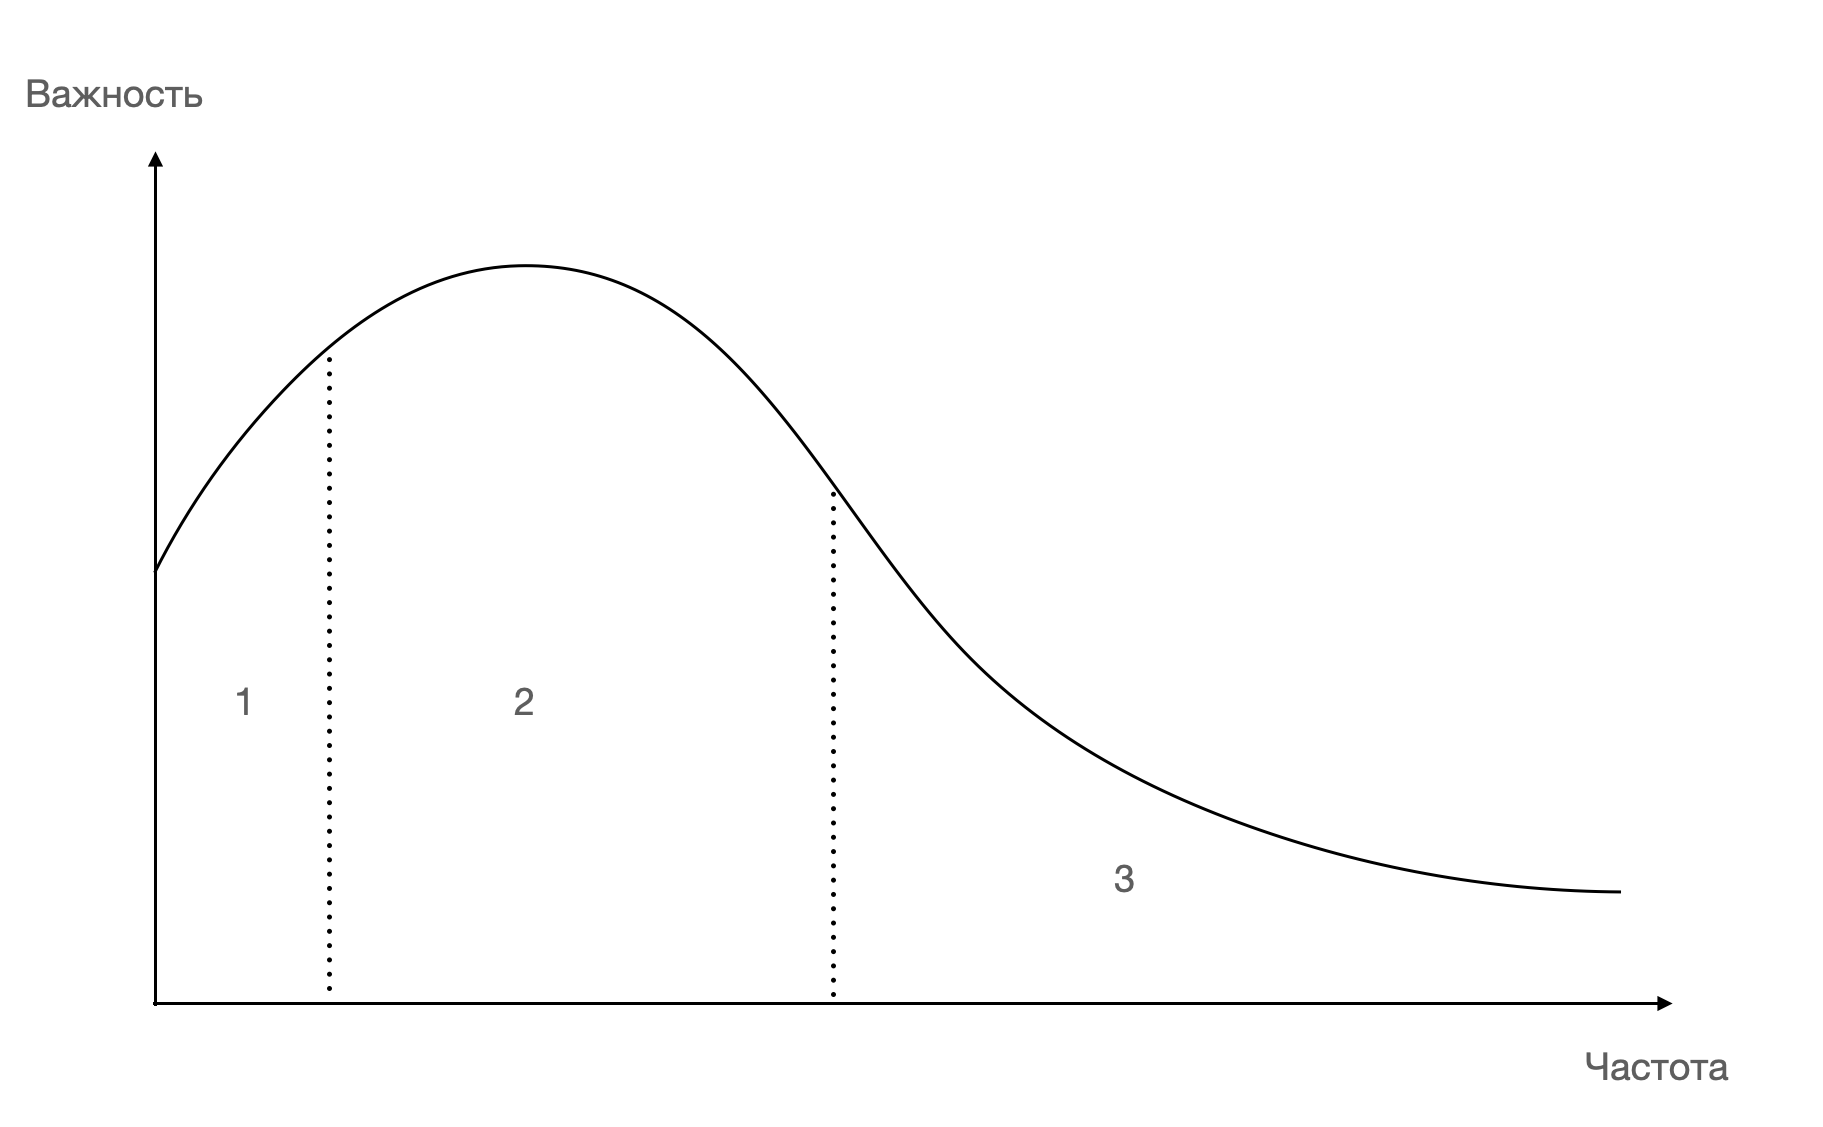
\includegraphics[width=0.5\linewidth]{13/Zipf}
Поэтому, в итоге, текст это вектор, где на i - ом месте стоит tf*idf слова $w_i$. Мера близости текстов A и B в векторной модели - косинус угла между векторами A и B.

\subsubsection {Морфологический анализ}
\href{http://prutzkow.com/ru-ru/science/natural-language-processing/morphology/}{Морфологический анализ} \\
Перед построением векторов сначала несколько унифицируют используемые слова, для этого используют морфологический анализ.
Морфологический анализ может быть словарным (со словарем основ и окончаний или словарем словоформ) или бессловарным (только со словарем окончаний; словарь окончаний может быть встроен в алгоритм морфологического анализа). Бессловарный метод используется только для определения переменной морфологической информации (не всегда однозначно), а словарный — во всех остальных случаях. 

\subsubsection {Исправление опечаток}
\href{https://ru.wikipedia.org/wiki/Расстояние_Левенштейна}{Расстояние по Левенштейну} \\
Элементарная операция по Левенштейну - это добавление буквы, удаление буквы или замена одной буквы на другую. Расстояние это количество операций необходимое для того, чтобы из одного слова получить другое с помощью операций Левенштейна. Например, слова aabb, aabbb, aab, aacb находятся на одинаковом расстоянии (расстояние равно 1). Далее, чтобы исправить опечатку необходимо найти ближайшее слово по Левенштейну.

\subsubsection {Поиск дубликатов}
Если необходимо решить задачу на полное совпадение текстов, то она делается очень просто. Для каждого документа берется хэш функция. С большой вероятностью документы с совпадающем хэшем - совпадают. Но на практике необходимо искать не в точности совпадающие тексты, а просто похожие. В таком случае используют понятие N-грамм.  \\
Определение: N-грамма — последовательность из n элементов. Например для текста: Мама мыла раму, все 4 граммы имеют вид: мама, амам, мамы, амыл, мыла, ылар, лара, арам, раму.  \\
Теорема. Если документы почти совпадают, то и N-граммы почти совпадают\\
Это отличный способ, сравнивать все N-граммы, но есть одна проблема - их очень много и сравнение всех N-грамм двух текстов займет много времени. Поэтому действуют следующим образом

\begin {itemize}
\item Берутся все N-граммы двух текстов и к ним применяется какой-нибудь хеш. (хэш функция от N - граммы называется называется шинглом)
\item Береться 84 шингла (значения хэш функции), они объединяются в 12 групп
\item На каждой группе шинглов опять вычисляется хэш функция. (значение хэш функции на группе шинглов называется супершинглом)
\item Если у двух текстов совпадает хотя бы один супершингл,  то они потенциально совпадают.
\end {itemize}

\subsubsection {Классификация и кластеризация}
Классификация - разделение на текстов группы, которые мы заранее определили. Кластеризация - разделение на группы, заранее не известные.
Примеры разделение: по авторству, по эмоциональной окраске текста, по цели (повествование/реклама), по различным темам.
Методы (одинаково применяются для кластеризации и классификации)

\begin {itemize}
\item Тезаурас. Берется двудольный граф, в котором в одной доле (будем ее называть доля  W) располагаются термины, а во второй доле - темы (будем ее называть T). Вершина из W соединяется с вершиной из T, когда соответсвующий термин описывает данную тему. Данный граф дается нам сверху лингвистами или еще кем то. Далее мы читаем полученный текст и считаем сколько раз встретился тот или иной термин. Термин, наиболее часто встречающийся, выбирается победителем и тема к которой он относится - тема текста. Минус этого метода: кто-то должен нам дать двудольный граф.
\item Самообучающиеся карты.
Пусть стоит задача разделить цветные точки на группы так, чтобы в каждой группе были точки одного цвета. В начальный момент времени все точки расположены в трехмерном пространстве хаотично (Почему трехмерном? Каждый цвет однозначно представляется тремя числами в системе rdb). Выбираются функции $f_1, f_2, f_3$ как показано на рисунке (Интеграл от них равен 1)
Далее используется следующий алгоритм:
\begin {itemize}
\item Для точки A в ее окрестности считается сумма $S = \sum_{p_i \in U} c (p_i) f_1 (\rho_i)$, где $U$ - окрестность точки A, $p_i$ - точки, принадлежащие этой окрестности, $c (p_i)$ - цвет точки $p_i$ (вектор в трехмерном пространстве), $\rho_i$ - расстояние от точки $p_i$ до точки A. Точка А красится в цвет S. Так последовательно делаем для всех точек.
\item Проделываем процедуру еще раз с функциями $f_2, f_3$
\item В итоге Все точки разделяться на группы.
\end {itemize}

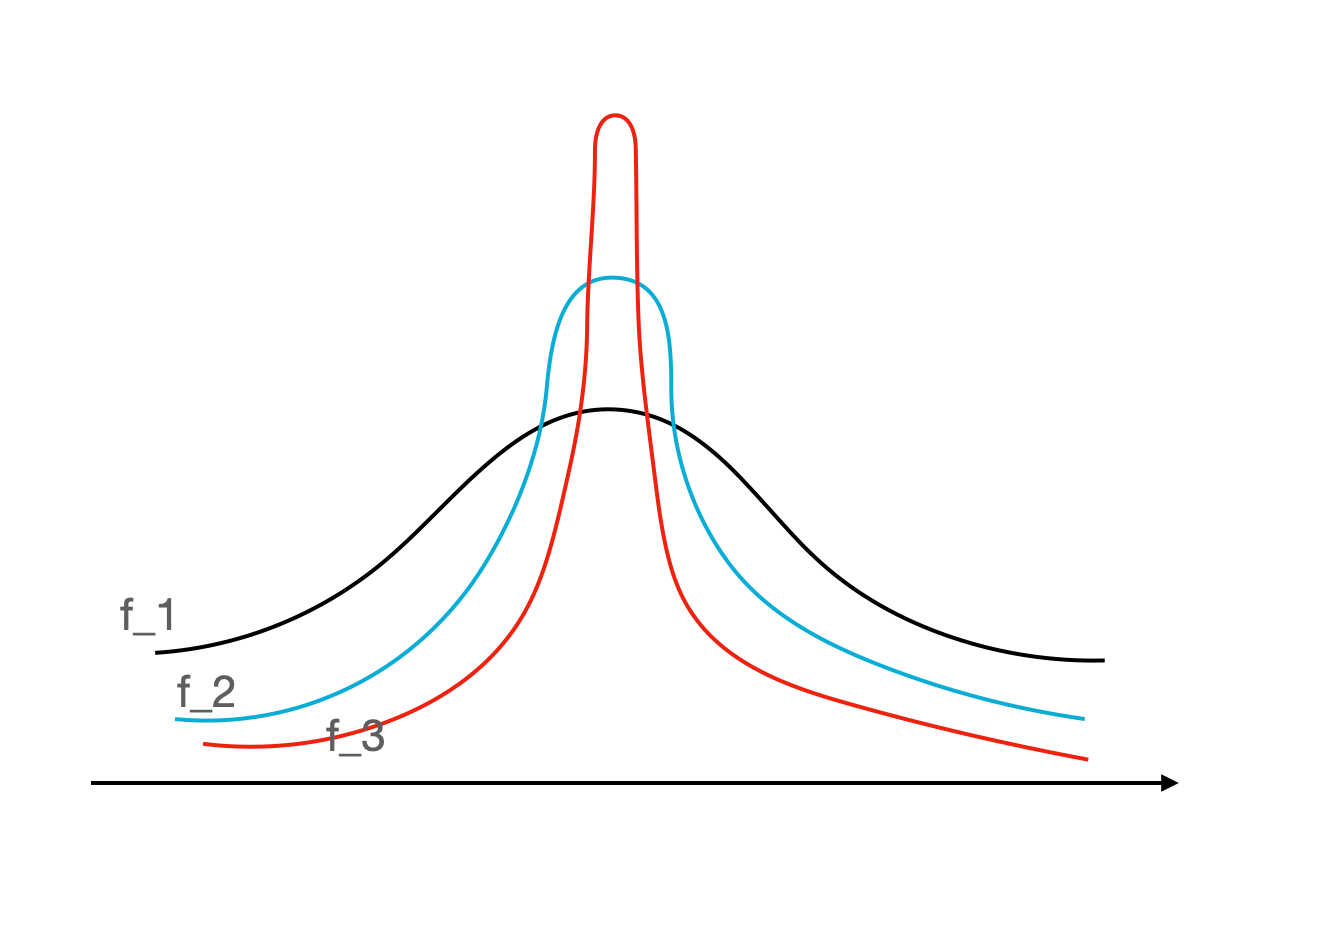
\includegraphics[width=0.5\linewidth]{13/func}

\begin{figure}[h!]
\begin{minipage}[h]{0.49\linewidth}
\center{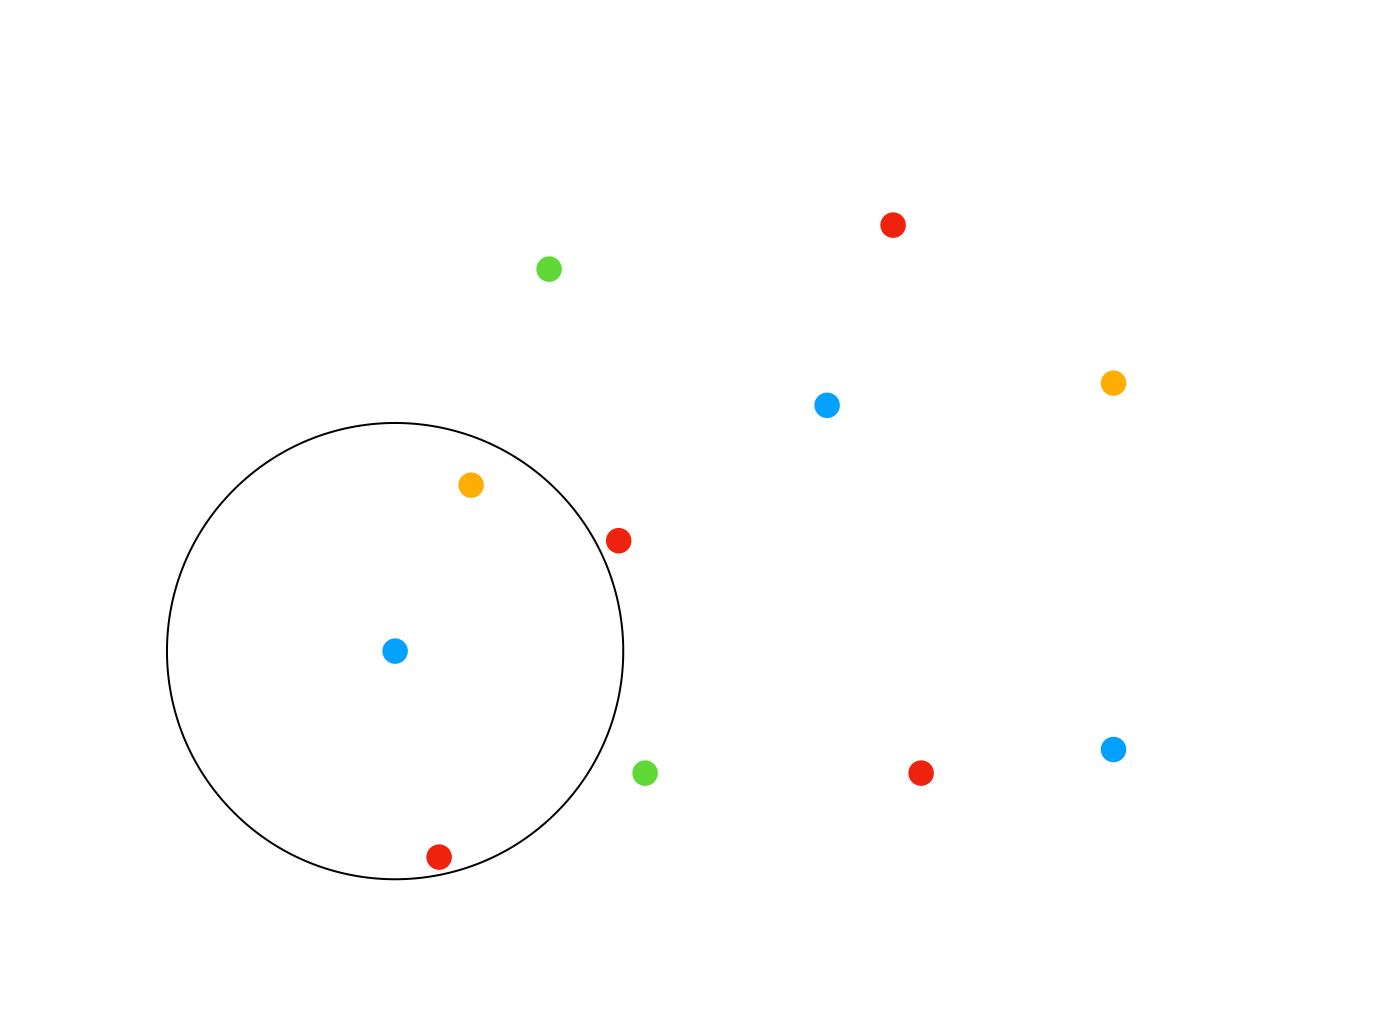
\includegraphics[width=\linewidth]{13/begin}}
\end{minipage}
\hfill
\begin{minipage}[h]{0.49\linewidth}
\center{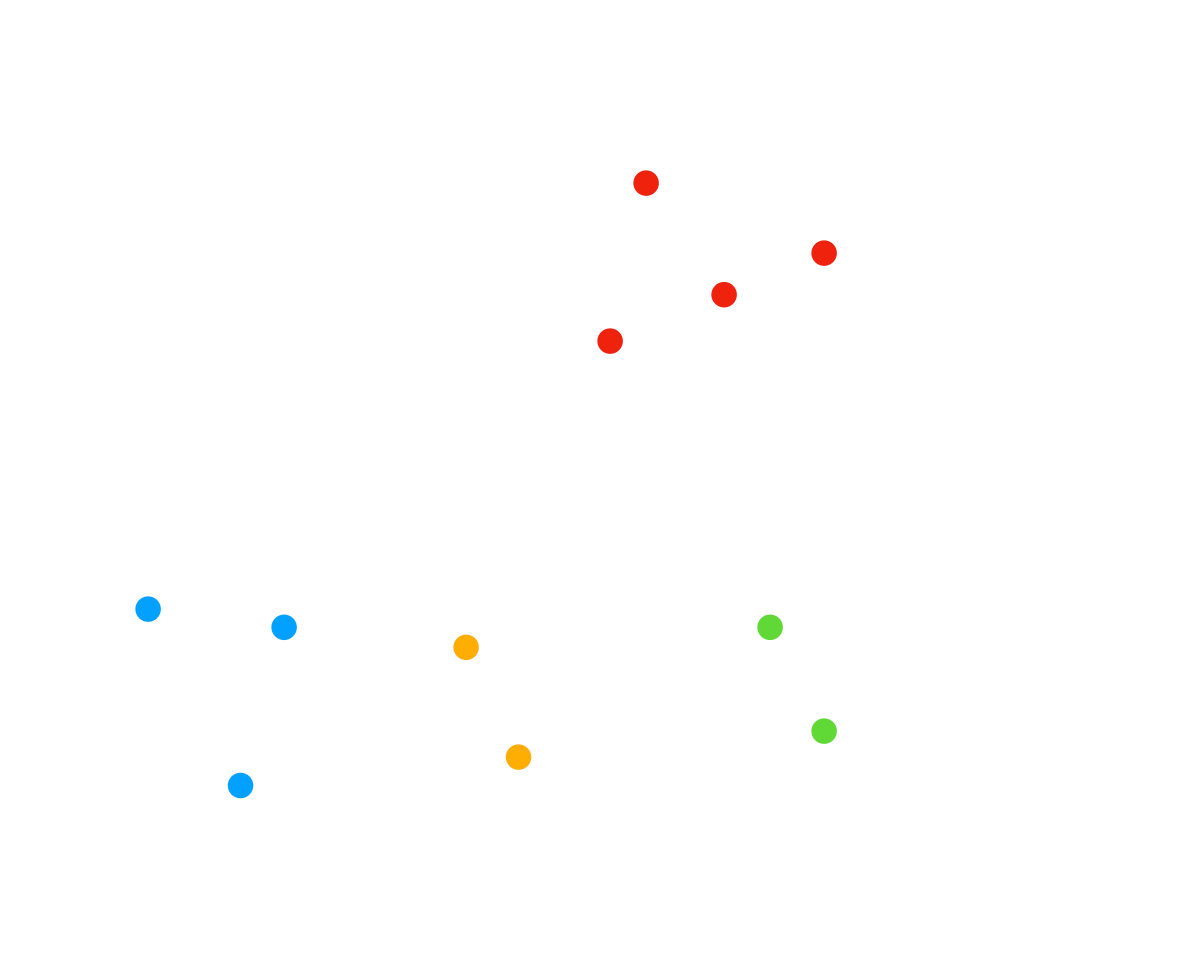
\includegraphics[width=\linewidth]{13/result}}
\end{minipage}
\end{figure}

\item  Физическая расстановка.
Стоит задача разделит точки на группы. Припишем каждой точке свою массу. Зададим векторы силы всемирного тяготения по формуле 
$\vec{F_{A,B}} = G \frac{m_{A} m_{B}\vec{r}}{|\vec{r}|^3}$, где $\vec{r}$ - вектор соединяющий точки А и В, $m_{A} m_{B}$ - массы точек. Тогда за время $\Delta t$ каждая точка под действием равнодейтсвующей силы притяжения передвинется на расстояние $\Delta s_i$ (свое для каждой точки). Если точки находятся близко, то объединяем их в одну точку суммарной массы. 

\item еще есть геометрическая расстановка \href{https://habr.com/ru/post/101338/}{habr.com}
\end{itemize} 



\subsubsection {Ранжирование}
Зачастую на запрос пользователя подходит несколько документов. Как выбрать один, наиболее подходящий? Для этого считают функцию ранжирования: $R = S A$, $S$ - функция соответствия запросу, A - функция авторитетности. 
\begin{itemize}
\item $S$ - функция соответствия запросу. Как обсуждалось выше это может быть косинус угла между текстом и запросом или например \href{https://ru.wikipedia.org/wiki/Okapi_BM25}{BM25}
\item A - функция авторитетности конкретного документа (эта функция своя для каждого документа и ее значение не зависит от запроса). Приведем пример определения авторитетности: Пусть есть ссылочный граф, т.е. в вершинах графа тексты и если текст A ссылается на текст B, то в графе есть соответсвующее ребро. Запустим в граф робота, который будет ходить по графу по следующему правилу, с вероятность p робот переходит из вершины в которой находится в одну из вершин на которую ссылается данная, и с вероятность (1 - р) - переходит в случайную вершину графа. Чем больше раз робот прошел через вершину, тем больше ее авторитетность.
\end {itemize}



